%%%% fatec-article.tex, 2024/03/10

%% Classe de documento
\documentclass[
  a4paper,%% Tamanho de papel: a4paper, letterpaper (^), etc.
  12pt,%% Tamanho de fonte: 10pt (^), 11pt, 12pt, etc.
  english,%% Idioma secundário (penúltimo) (>)
  brazilian,%% Idioma primário (último) (>)
]{article}

%% Pacotes utilizados
\usepackage[]{fatec-article}
\Author{1}{Name={Autor 1\\ Autor 2 \\ Autor 3\\ Autor 4}}

\Author{2}{Name={\{ autor1@fatec.sp.gov.br \}\\ \{ autor2@fatec.sp.gov.br \} \\ \{ autor3@fatec.sp.gov.br\} \\ \{ autor4@fatec.sp.gov.br \}}}

%% Definição das palavras-chaves/keywords
\Keyword{1}{Artigo}{Article}
\Keyword{2}{Latex}{Latex}
\Keyword{3}{Informática}{Informatic}

%%%% Resumo no idioma primário (brazilian)
\begin{Abstract}[brazilian]%% Idioma (brazilian ou english)
  O resumo FATEC Registro é uma descrição completa e concisa dos componentes-chave da metodologia do estudo e dos achados importantes da pesquisa. Normalmente, o resumo é o primeiro encontro do leitor com uma pesquisa ou relato, sendo algumas vezes o único elemento recuperado e/ou revisado nas bases de dados científicos. Esse elemento provê a primeira impressão, muitas vezes a mais importante, identificando o valor potencial ou a relevância do enfoque da pesquisa e dos resultados. Se o resumo for bem escrito, ele atrairá leitores para obter uma cópia do manuscrito completo que será incorporado aos que já foram encontrados, e seu trabalho será citado. Se o resumo for mal escrito, a pesquisa poderá ser ignorada ou, até mesmo, esquecida.
\end{Abstract}

%%%% Resumo no idioma secundário (english)
\begin{Abstract}[english]%% Idioma (brazilian ou english)
The summary is a complete and concise description of the key components of the study methodology and important research findings. Typically, the summary is the reader's first encounter with a research report or paper, and sometimes it is the only element retrieved and/or reviewed in scientific databases. This element provides the first impression, often the most important one, identifying the potential value or relevance of the research approach and findings. If the summary is well-written, it will attract readers to obtain a copy of the full manuscript that will be incorporated into those already found, and your work will be cited. If the summary is poorly written, the research may be ignored or even forgotten.
\end{Abstract}

%% Processamento de entradas (itens) do índice remissivo (makeindex)
\makeindex%

%% Arquivo(s) de referências
\addbibresource{fatec-article.bib}

%% Início do documento
\begin{document}

% Seções e subseções
%\section{Título de Seção Primária}%

%\subsection{Título de Seção Secundária}%

%\subsubsection{Título de Seção Terciária}%

%\paragraph{Título de seção quaternária}%

%\subparagraph{Título de seção quinária}%

\section*{Introdução}%
\label{sect:intro}
Atualmente existem hoje no mundo 58.497 espécies de árvores, sendo que a região da américa latina compreende a distribuição de 23.631 espécies.\cite{bgci}

Contudo, entre os anos de 2020 e 2021 foram desflorestados 21.642 ha. da Mata Atlântica brasileira, equivalente a mais de 28000 campos de futebol. Os dados foram apresentados no Atlas dos Remanescentes Florestais da Mata Atlântica, uma colaboração entre o Instituto de Pesquisas Espaciais(INPE) e a Fundação SOS Mata Atlântica. O Relatório Anual de 2022 também indica que este foi o valor foi o mais alto desde 2015 e 90\% maior do que o menor valor da história, alcançado em 2018.\cite{atlas-mata-atlantica}

Segundo um levantamento feito  em 2020 pelo MapBiomas, uma rede Colaborativa que mapeia anualmente a cobertura e uso do solo,apenas 29,7\% do total do bioma Mata Atlântica tem formação Florestal.\cite{mapbiomas}

O Ministério do Meio Ambiente, baseando-se na classificação de risco de extinção do BGCI, por intermédio da portaria Nº 43 de 31 de janeiro de 2014 \cite{mma2014},  Institui o Programa Nacional de Conservação das Espécies Ameaçadas de Extinção - Pró-Espécies. A portaria Nº 443 de 17 de dezembro de 2014\cite{mma20142}, atualiza a lista de espécies de plantas em risco de extinção, atualizada novamente pela portaria Nº 148 de 7 de junho de 2022.\cite{mma2022}

Associado ao desmatamento está a perda da biodiversidade das espécies de plantas. Dados do Botanic Gardens Conservation International(BGCI), demonstram que 30\% das espécies de árvores da américa latina encontram-se ameaçadas de extinção.\cite{bgci}

Com o intuito de guiar e coordenar o desenvolvimento sustentável no mundo, as Organizações das Nações Unidas idealizaram os 17 Objetivos de Desenvolvimento Sustentável, para erradicação da pobreza, proteção do meio ambiente e clima. Dentre esses objetivos, destacamos a ODS 15 que visa proteger, restaurar e promover o uso sustentável de ecossistemas terrestres bem como gerenciar florestas de forma sustentável. Assim, proteger as florestas nativas e ecossistemas de serem degradados impactam diretamente nas ações Globais contra a Mudança do Clima, objeto da ODS 13. Ainda, segundo o relatório MapBiomas, 70\% da Mata Atlântica tem uso antrópico sendo esta a prioridade da ODS 11, que busca tornar assentamentos humanos seguros e sustentáveis.\cite{agenda2030}

No decorrer deste estudo será realizada a identificação de uma espécie arbórea de nome científico \textit{Cecropia pachystachya}, popularmente conhecida como Embaúba. Segundo Carvalho (2006) em seu manual de Espécies Arbóreas, a Embaúba é uma árvore perenifólia que atinge cerca de 25 metros de altura e 45 centímetros de DAP (diâmetro à altura do peito, medido a 1,30m do solo) em sua fase adulta. Seu tronco é reto, cilíndrico e fistuloso (oco por dentro). A casca externa é áspera e cinza-clara, com até 6mm de espessura, enquanto a casca interna é alaranjada-rosada e fibrosa. Suas folhas são alternadas e agrupadas nas extremidades dos ramos, com lâmina de 20 a 35 cm de comprimento por 20 a 35 cm de largura. Elas são palmatilobadas e divididas em 5 a 12 lobos desiguais obovados, separados até o pecíolo por espaços de 2 a 3 cm, e densamente esbranquiçadas-tomentosas na face inferior. A face superior apresenta pelos curtos e esparsos, margem inteira ou ligeiramente ondulada e ápice obtuso, com nervura central proeminente na face inferior. O pecíolo é forte e comprido, medindo de 16 a 25 cm de comprimento, com pelos uncinados e cálix na base. É uma espécie dióica, ou seja, possui indivíduos machos e fêmeas.\cite{carvalho2006embauba}
A Embaúba é uma espécie pioneira, associada a capoeiras novas, situadas junto a vertentes ou cursos d'água, estabelecendo-se rapidamente em clareiras descampadas. Popularmente é conhecida por seu uso medicinal da folha e casca. \cite{carvalho2006embauba}

Andrade et. al avaliaram o potencial antimicrobiano e antifúngico do extrato etanólico de folhas da Embaúba, que demonstrou atividade contra linhagens bacterianas \textit {Staphylococcus aureus}, \textit {Streptococcus pyrogenes} e a levedura Candida albicans levando a resultados promissores.\cite{de2021avaliaccao}

No presente trabalho, será usada a classificação de risco, desenvolvido pela Lista Vermelha da IUCN, um sistema destinado a classificar espécies em alto risco de extinção global e de forma amplamente compreensível. Utiliza procedimentos de avaliação padronizados para atribuir espécies a diferentes categorias de risco de extinção com base em cinco critérios quantitativos, incluindo medidas de tamanho populacional, restrição de distribuição geográfica e taxa de declínio.  (IUCN Red List, 2021)
No Brasil, a classificação da lista Vermelha é adotada pelo Ministério do Meio Ambiente através da portaria Nº 148 de 7 de junho de 2022, que lista as espécies de plantas em risco de extinção dos biomas brasileiros. (MMA, 2022)

A partir dessa classificação será possível classificar espécies quanto o seu grau de risco de extinção e, num segundo momento, propor ações de manejo sustentável a fim de rastrear as espécies de árvores alvo da pesquisa, para esse fim será utilizado o sistema de coordenadas SIRGAS.\par

O SIRGAS (Sistema de Referência Geodésico para as Américas) é um sistema de referência geodésico associadas a uma determinada época de referência e a sua variação ao longo do tempo é tomada em consideração, seja pelas velocidades individuais das estações, ou por um modelo de velocidade contínuo que compreende os movimentos das placas litosféricas e as deformações na crosta. \cite{SIRGAS2023}

Para a coleta de dados em campo, foi empregada a escala de Likert como método de obtenção de informações. Essa técnica é reconhecida e frequentemente utilizada em pesquisas científicas, permitindo que os participantes expressem suas opiniões, atitudes ou experiências em relação a variáveis específicas de interesse. A escala de Likert consiste em uma série de afirmações ou questões nas quais os respondentes atribuem um grau de concordância ou discordância, geralmente em uma escala que varia de "discordo totalmente" a "concordo totalmente", com diferentes níveis intermediários.  Segundo Nogueira (2002), essa abordagem oferece uma maneira estruturada e quantificável de coletar dados sobre uma ampla variedade de fenômenos, fornecendo insights valiosos para análises posteriores. Essa escala pode ser adaptada com diferentes quantidades de pontos ou níveis de detalhamento, visto que um número maior de pontos proporciona respostas mais precisas.

De forma  contribuir com gestão dos recursos florestais de forma a reduzir o desmatamento e garantir a preservação das espécies de árvores brasileiras, o presente trabalho tem como objetivo desenvolver um Sistema Web para identificação de flora por imageamento aéreo utilizando Inteligência Artificial (IA), capaz de identificar árvores de interesse econômico e ambiental, importantes para equilíbrio da biodiversidade, bem como espécies invasoras, que podem implicar na perda da biodiversidade, além de identificar espécies em risco de extinção. A aplicação destina-se à elaboração de inventários florestais, em projetos de empreendimentos imobiliários, bem como embasamento técnico para propostas de manejo e rastreamento de árvores na região da mata Atlântica.

\section*{OBJETIVO} \label{sect:obj}

O objetivo do presente trabalho foi desenvolver uma aplicação baseada em redes neurais convolucionais (CNN) para identificação automatizada da Cecropia pachystachya (embaúba) em imagens aéreas, visando otimizar o processo de reconhecimento dessa espécie na Mata Atlântica e contribuir para a conservação da biodiversidade. Assim, o trabalho visa:

\begin{itemize}
\item Criar um sistema de identificação capaz de detectar a embaúba em larga escala, auxiliando no monitoramento de áreas de interesse ambiental.
\item Facilitar a elaboração de laudos de flora com maior precisão e eficiência.
\item Gerar relatórios automatizados, permitindo o rastreamento de espécies nativas e invasoras.
\item Disponibilizar relatórios dinâmicos para apoiar a tomada de decisões em manejo ambiental e políticas de preservação.
\end{itemize}







\section*{ESTADO DA ARTE} \label{sect:estadoarte}

A identificação de árvores de interesse ambiental e econômico torna-se um desafio em grandes áreas, especialmente devido à dificuldade de distinguir entre espécies com características semelhantes. A utilização de aprendizado profundo e Inteligência Artificial pode otimizar esse processo, tornando-o mais rápido, eficiente e com alta acurácia. Essa abordagem tecnológica possibilita a geração de dados confiáveis para subsidiar tomadas de decisão e a elaboração de estratégias de manejo sustentável.
Para classificar e mapear plantas ameaçadas na Mata Atlântica de forma colaborativa, de Souza et al. (2020) desenvolveram um aplicativo baseado em uma arquitetura MobileNet adaptada. Os autores utilizaram imagens da Encyclopedia of Life, ampliadas através de data augmentation (com filtros verticais e horizontais), distribuídas em conjuntos de treinamento (70\%), validação (20\%) e teste (10\%). O modelo foi treinado por 23 épocas com taxa de aprendizado de 0,00001 e função de ativação ReLU, empregando transfer learning em blocos convolucionais selecionados. A abordagem demonstrou alta acurácia e baixa taxa de erro nos três blocos de convolução mais eficientes. Em seus experimentos, realizados no município de Jacareí-SP, alcançaram uma acurácia superior a 90\% para as espécies Araucária e 99,9\% para as espécies de Pitanga.
No estudo de Carneiro (2023), desenvolveu-se um modelo de Deep Learning para identificação de Aspidosperma polyneuron (Peroba-Rosa) em fragmentos florestais, utilizando imagens de sensoriamento remoto integradas a técnicas de machine learning. Os dados de referência foram obtidos por meio de um inventário florestal prévio, que mapeou a localização exata de 302 indivíduos distribuídos em 126 hectares. Desse total, 100 indivíduos foram utilizados para treinamento do modelo e os demais para validação. Aplicou-se a técnica de data augmentation para ampliar artificialmente o conjunto de treinamento, gerando 1.162 amostras adicionais. O modelo empregado consistiu em uma Regional Convolutional Neural Network (R-CNN) da biblioteca ESRI, treinada com 10 épocas. Os resultados indicaram precisão de 23\% e acurácia de 71\% na avaliação de novos indivíduos, sugerindo a necessidade de aprimoramentos em pesquisas futuras para otimizar o desempenho do modelo.
Diante dos avanços promissores apresentados pelos estudos de de Souza et al. (2020) e Carneiro (2023), fica evidente a necessidade de ampliar pesquisas que explorem diferentes aspectos de treinamento de modelos de IA, como arquiteturas variadas, técnicas de aumento de dados e estratégias de transfer learning, visando superar os desafios de identificação de espécies em ambientes complexos. A otimização dessas ferramentas tecnológicas não só elevaria a precisão dos resultados, como também reforçaria seu impacto ecológico ao permitir o monitoramento eficiente de espécies ameaçadas e o planejamento de ações de conservação. Além disso, o aprimoramento desses sistemas traria significativos benefícios econômicos, viabilizando o manejo sustentável de recursos florestais valiosos e a geração de dados confiáveis para políticas públicas e iniciativas privadas.


\section*{METODOLOGIA} \label{sect:metodologia}

A seção de Metodologia explica aos leitores quais procedimentos, abordagens, desenhos e tratamento realizamos na pesquisa, o que permitirá replicar os estudos, entender a linearidade entre a abordagem dos objetivos e os resultados obtidos, determinar sua adequação e relevância e evidenciar qualquer viés na maneira como o estudo foi elaborado e realizado. Em outras palavras, é uma estrutura contextual que apresenta um caminho lógico para responder a perguntas que você levanta no início de sua tese ou artigo \cite{knuth:84}. 

É importante que nesta seção, você descreva todas as ferramentas e tecnologias utilizadas para o desenvolvimento da sua pesquisa \cite{boulic:91}. Lembre-se de detalhar para que serve cada ferramenta e tecnologia e o motivo da sua escolha.


\section*{RESULTADOS PRELIMINARES}\label{sect:resultados}

\subsection*{PESQUISA DE CAMPO E ANÁLISE ESTATÍSTICA}

A pesquisa de campo foi desenvolvida por meio de questionário, contendo quatro perguntas que avaliam a adoção de novas tecnologias no campo da preservação do meio ambiente. Foram feitas nove entrevistas em órgãos públicos como CETESB e Fundação Florestal, bem como um escritório de Engenharia Ambiental.
A primeira pergunta buscava conhecer se aquele órgão ou empresa estava ligado e comprometido com a preservação do meio ambiente, e foi obtido resposta positiva 100\% das entrevistas.
A segunda pergunta busca avaliar se na opinião do entrevistado, o custo envolvido na realização de um levantamento de flora, é uma barreira para usa execução. 22\% dos entrevistados responderam que não é uma barreira, enquanto os outros 78\% concordam que o custo é um fator importante na realização desse serviço.
\Cref{Gráfico 1}
\begin{figure}[!h]
    \centering
    \caption{Respostas tabuladas}
    \label{Gráfico 1}
    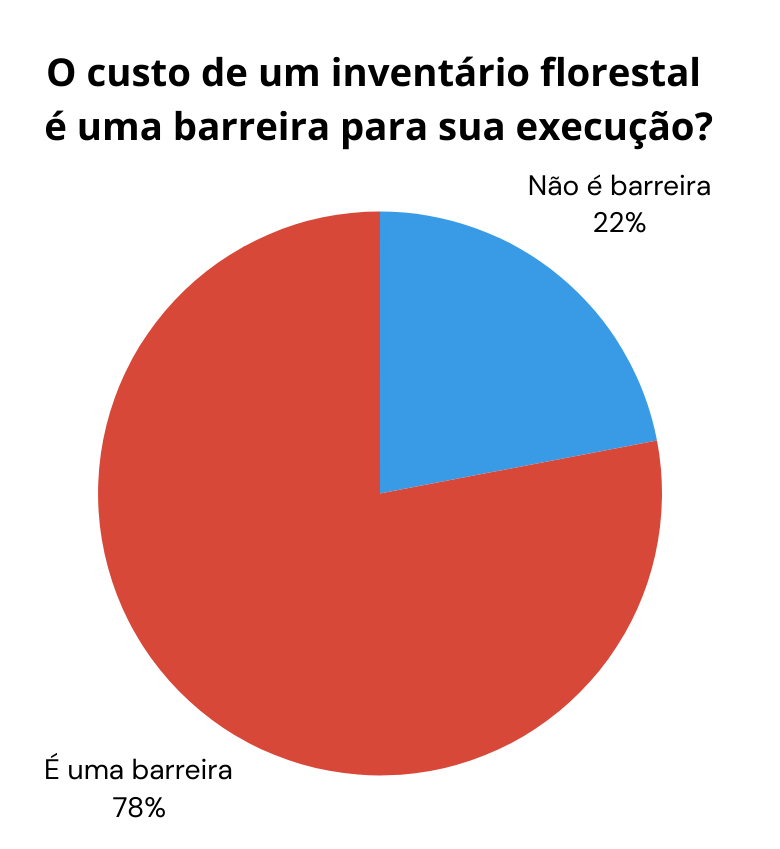
\includegraphics[width=0.5\linewidth]{Illustrations/grph-question2.png}
    \SourceOrNote{Autoria Própria (2024)}
    \end{figure}

Na terceira pergunta levantou-se a disponibilidade de ferramentas tecnológicas que auxiliem a preservação de árvores no meio ambiente. Um entrevistado respondeu que no seu setor não dispunha de quaisquer recursos, ainda que necessários. Todos os outros responderam que possuem tecnologias das mais diversas: Drones, Aerofotos, Mapa de Arborização urbana (Online), GPS, Google Earth, Sobrevoo de helicóptero, plataforma ArcGis, MITRA, Cartas Topográficas, máquina fotográfica, banco de dados diversos.
A quarta pergunta investigou o nível de confiança dos entrevistados em análises feitas por IA como auxílio para tomadas de decisão nas funções que desempenham. 44\% dos entrevistados responderam não confiar em análises feitas por IA, entretanto 56\% acreditam que ela possa ser usada como ferramenta para auxiliar tomadas de decisões.
\Cref{Gráfico 2}
\begin{figure}[!h]
    \centering
    \caption{Respostas tabuladas}
    \label{Gráfico 2}
    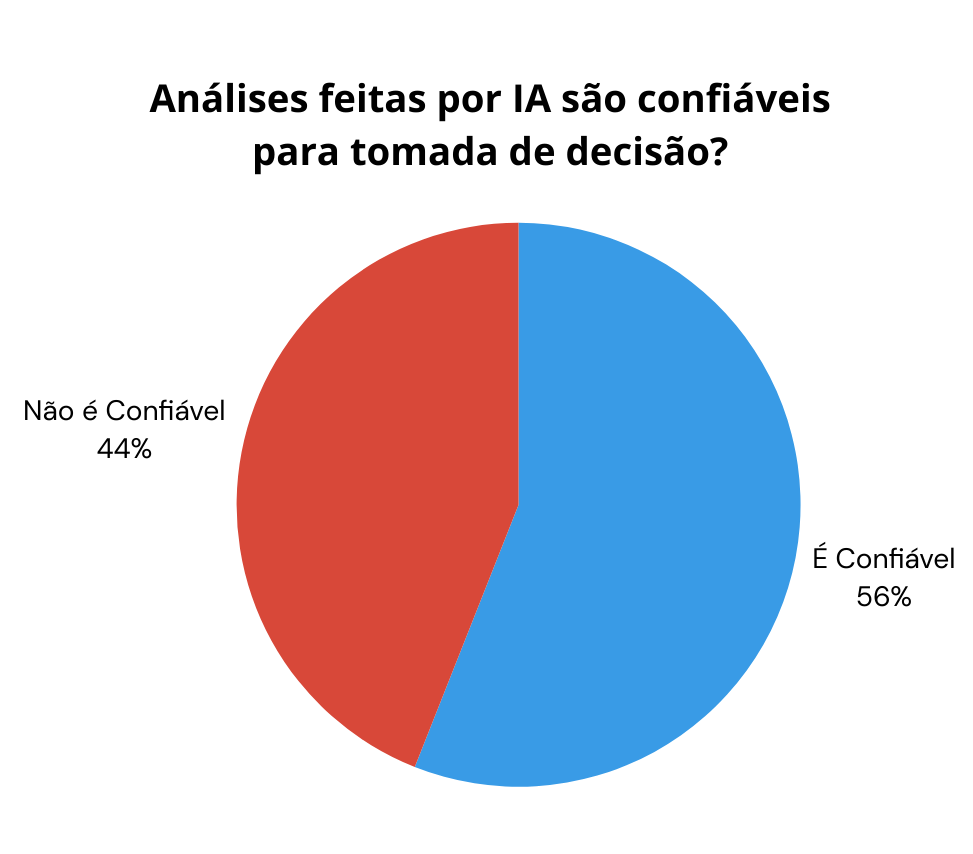
\includegraphics[width=0.65\linewidth]{Illustrations/pizza2.png}
    \SourceOrNote{Autoria Própria (2024)}
    \end{figure}

A pesquisa nos revelou que existe uma carência de ferramentas tecnológicas de monitoramento e imageamento aéreo. Isso é evidenciado no uso frequente de aerofotos antigas e cartas topográficas impressas. Pela falta desses recursos, o levantamento de espécies para um inventário florestal resulta em um serviço de alto custo, e que são feitos somente em caso de extrema necessidade. Essa situação reflete na visão que os profissionais têm sobre as IA's, em que as respostas ficaram divididas entre se elas são viáveis ou não para tomadas de decisão.

\subsection*{DESEMPENHO DO MODELO}
Resultados da Validação Cruzada
O desempenho do modelo foi avaliado utilizando validação cruzada (K-Fold Cross Validation) com 10 folds. A seguir estão os resultados de acurácia de validação para cada fold:

Fold 1: 92.5\%

Fold 2: 85.0\%

Fold 3: 85.0\%

Fold 4: 90.0\%

Fold 5: 87.5\%

Fold 6: 80.0\%

Fold 7: 82.5\%

Fold 8: 82.5\%

Fold 9: 77.5\%

Fold 10: 82.5\%

\subsubsection*{Análise da Acurácia Média}

A acurácia média de validação obtida ao longo dos 10 folds foi de 84.5\%, indicando um bom desempenho do modelo na tarefa de classificação. Esta métrica reflete a capacidade do modelo de generalizar bem para novos dados.

\subsubsection*{Variabilidade entre os Folds}

Houve alguma variação nos resultados de acurácia entre os diferentes folds, com um mínimo de 77.5\% e um máximo de 92.5\%. Esta variabilidade é esperada devido a diferenças na distribuição dos dados em cada fold e sugere que, enquanto o modelo performa consistentemente bem, há espaço para melhorias na generalização.\Cref{Gráfico 3}

O modelo foi treinado por 100 épocas com um batch size de 32, usando o otimizador Adam e a função de perda sparse\textunderscore categorical\textunderscore crossentropy. Este número de épocas foi suficiente para permitir ao modelo aprender as características dos dados sem superajustar aos dados de treinamento. A função de ativação ReLU nas camadas densas e softmax na camada de saída ajudaram a capturar relações não-lineares e a classificar corretamente as imagens.

\begin{figure}[!h]
    \centering
    \caption{Evolução da acurácia ao longo dos treinamentos}
    \label{Gráfico 3}
    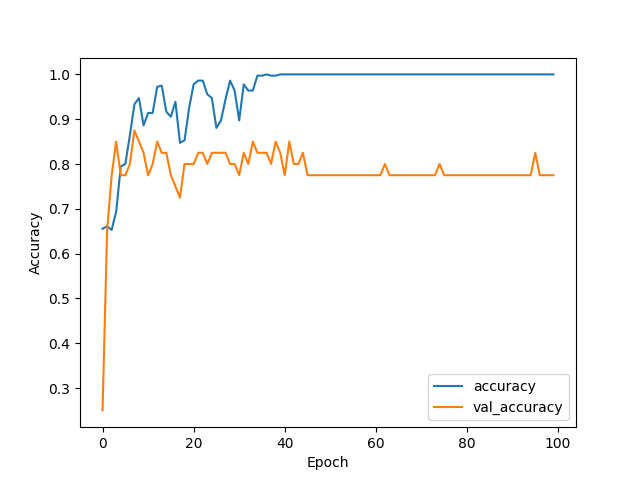
\includegraphics[width=0.7\linewidth]{Illustrations/Figure_1.png}
    \SourceOrNote{Autoria Própria (2024)}
    \end{figure}

\section*{CONCLUSÃO}\label{sect:conclusao}

A proposta do sistema web é promissora, pois utiliza inteligência artificial para analisar imagens aéreas em larga escala, automatizando processos que requerem recursos humanos e técnicos avançados.
Essa abordagem permite a geração de laudos com altas taxas de acurácia, que podem ser utilizados em relatórios técnicos científicos, e mesmo resultados menos precisos podem auxiliar na identificação de espécies em extinção. Além disso, o baixo custo dessas análises pode desempenhar um papel decisivo na tomada de decisões e auxiliar o poder público a automatizar processos de cálculos de Restauração de Flora.
O alto nível de acurácia obtido, acima de 80\% indica um bom desempenho do modelo na tarefa de classificação, refletindo a capacidade do modelo em generalizar novos dados.
A proposta do aplicativo é promissora, pois utiliza inteligência artificial para analisar imagens aéreas em larga escala, automatizando processos que requerem recursos humanos e técnicos avançados. Essa abordagem permite a geração de laudos com altas taxas de acurácia, que podem ser utilizados em relatórios técnicos científicos, e mesmo resultados menos precisos podem auxiliar na identificação de espécies em extinção. Além disso, o baixo custo dessas análises pode desempenhar um papel decisivo na tomada de decisões em projetos de recuperação da flora nativa e restauração de ambientes degradados por desmatamento.

\printbibliography

%% Elementos pós-textuais (opcionais): Apêndice e Anexo
%Caso for utilizar, basta retirar o símbolo de % na frente do comando
%%%%% Elementos pós-textuais
%%
%% Glossário, apêndices, anexos e índice remissivo (opcionais).

%% Apêndices
\begin{Appendix}

\section{Título de Apêndice}%
\label{sect:apx-a1}

Exemplo de apêndice (\Cref{sect:apx-a1}) em uma seção de \nameref{sect:appendix}.

\subsection{Título de Seção Secundária de Apêndice}%
\label{ssect:apx-a2}

Exemplo de seção secundária de apêndice (\Cref{ssect:apx-a2}).

\subsubsection{Título de Seção Terciária de Apêndice}%
\label{sssect:apx-a3}

Exemplo de seção terciária de apêndice (\Cref{sssect:apx-a3}).

\paragraph{Título de seção quaternária de Apêndice}%
\label{prgh:apx-a4}

Exemplo de seção quaternária de apêndice (\Cref{prgh:apx-a4}).

\subparagraph{Título de seção quinária de Apêndice}%
\label{sprgh:apx-a5}

Exemplo de seção quinária de apêndice (\Cref{sprgh:apx-a5}).

\end{Appendix}

%% Anexos
\begin{Annex}

\section{Título de Anexo}%
\label{sect:anx-a1}

Exemplo de anexo (\Cref{sect:anx-a1}) em uma seção de \nameref{sect:annex}.

\subsection{Título de Seção Secundária de Anexo}%
\label{ssect:anx-a2}

Exemplo de seção secundária de anexo (\Cref{ssect:anx-a2}).

\subsubsection{Título de Seção Terciária de Anexo}%
\label{sssect:anx-a3}

Exemplo de seção terciária de anexo (\Cref{sssect:anx-a3}).

\paragraph{Título de seção quaternária de Anexo}%
\label{prgh:anx-a4}

Exemplo de seção quaternária de anexo (\Cref{prgh:anx-a4}).

\subparagraph{Título de seção quinária de Anexo}%
\label{sprgh:anx-a5}

Exemplo de seção quinária de anexo (\Cref{sprgh:anx-a5}).

\end{Annex}

%% Índice remissivo
\printindex%


%% Fim do documento
\end{document}